\documentclass[11pt]{article}
\usepackage{cornell-notes}
\usepackage{mathtools}
\usepackage{needspace}
\usepackage{ragged2e}
\usepackage{adjustbox}
\usepackage{tikz}
\usetikzlibrary{arrows.meta,positioning}
\tcbuselibrary{most}
\geometry{letterpaper,margin=0.72in,headheight=15pt}
\setCornellCollection{Calculus Cornell Notes}
\setCornellUnitType{Chapter}
\setCornellUnitNumber{5}
\setCornellUnitTitle{Logarithmic, Exponential, and Other Transcendental Functions}

\definecolor{Ink}{HTML}{17324D}
\definecolor{Teal}{HTML}{147D78}
\definecolor{Sky}{HTML}{DDEEF1}
\definecolor{Cue}{HTML}{EEF2F5}
\definecolor{Warm}{HTML}{FFF3D6}
\definecolor{Alert}{HTML}{9D3C32}
\definecolor{Green}{HTML}{276749}
\definecolor{Rule}{HTML}{AAB8C2}
\hypersetup{colorlinks=true,linkcolor=Ink,urlcolor=Teal,pdfborder={0 0 0}}
\setlength{\parindent}{0pt}
\setlength{\parskip}{4pt}
\setlist{nosep,leftmargin=*}
\titleformat{\section}{\Large\bfseries\color{Ink}}{}{0pt}{}[\color{Teal}\titlerule]
\titleformat{\subsection}{\large\bfseries\color{Teal}}{}{0pt}{}
\pagestyle{fancy}
\fancyhf{}
\fancyhead[L]{\small\color{Ink}\textsc{Cornell Notes}}
\fancyhead[R]{\small\color{Teal}\nouppercase{\leftmark}}
\fancyfoot[L]{\footnotesize\color{Ink}Active recall $\bullet$ Worked reasoning $\bullet$ Verification}
\fancyfoot[R]{\footnotesize\color{Ink}\thepage\ of \pageref*{LastPage}}
\renewcommand{\headrulewidth}{0.5pt}
\renewcommand{\footrulewidth}{0.4pt}
\newcolumntype{Y}{>{\RaggedRight\arraybackslash}X}
\newtcolorbox{orientationbox}{enhanced,breakable,colback=Sky,colframe=Teal,boxrule=0.7pt,arc=2mm,title=Chapter orientation,fonttitle=\bfseries}
\newtcolorbox{sectionsummarybox}{enhanced,breakable,colback=white,colframe=Teal,boxrule=0.6pt,arc=1.5mm,left=2mm,right=2mm,top=1mm,bottom=1mm,title=Section synthesis,fonttitle=\bfseries\color{Teal}}
\newtcolorbox{warningbox}{enhanced,breakable,colback=Warm,colframe=Alert,boxrule=0.7pt,arc=1.5mm,title=Common error audit,fonttitle=\bfseries}
\newtcolorbox{checkbox}{enhanced,breakable,colback=white,colframe=Green,boxrule=0.7pt,arc=1.5mm,title=Verification habit,fonttitle=\bfseries}
\newcommand{\cornellcuehead}{\rowcolor{Ink}\color{white}\bfseries Cue / recall prompt & \color{white}\bfseries Notes / reasoning \\\endhead}
\newcommand{\cornellcuerow}[2]{\rowcolor{Cue}#1 & #2 \\\addlinespace[3pt]}
% Table-safe: delegates to the shared Cornell formula box (cornell-notes.sty),
% which cannot emit \pagebreak/\noalign inside longtable cells.
\newcommand{\formula}[1]{\CornellFormula[colback=Sky,colframe=Teal]{#1}}

\title{Chapter 5: Logarithmic, Exponential, and Other Transcendental Functions\\[2mm]\large Cornell Notes}
\author{}
\date{}
\hypersetup{pdftitle={Chapter 5: Logarithmic, Exponential, and Other Transcendental Functions - Cornell Notes},pdfauthor={},pdfsubject={Calculus study notes},pdfkeywords={calculus, Cornell notes, active recall}}
\begin{document}
\maketitle
\thispagestyle{fancy}
\begin{orientationbox}
Extend calculus to logarithmic, exponential, inverse trigonometric, and hyperbolic functions while respecting domains and inverse-function structure. These notes follow the complete local section sequence (313--404) and emphasize definitions, governing results, strategy selection, and verifiable reasoning.
\end{orientationbox}

\section{Prerequisite map}
\begin{minipage}[t]{0.42\textwidth}
\textbf{Bring forward}
\begin{itemize}
\item Chain Rule
\item Implicit differentiation
\item Integration by substitution
\item One-to-one functions
\end{itemize}
\end{minipage}\hfill
\begin{minipage}[t]{0.54\textwidth}
\textbf{Chapter flow}
\begin{center}
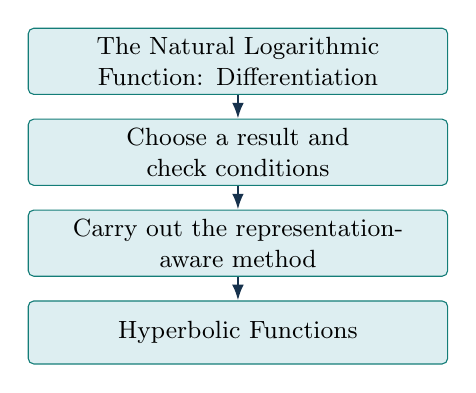
\begin{tikzpicture}[node distance=3mm, every node/.style={font=\small,align=center}, box/.style={draw=Teal,rounded corners=2pt,fill=Sky,minimum height=8mm,text width=0.42\textwidth}, arr/.style={-{Latex[length=2mm]},thick,draw=Ink}]
\node[box] (a) {The Natural Logarithmic Function: Differentiation};
\node[box,below=of a] (b) {Choose a result and check conditions};
\node[box,below=of b] (c) {Carry out the representation-aware method};
\node[box,below=of c] (d) {Hyperbolic Functions};
\draw[arr] (a)--(b); \draw[arr] (b)--(c); \draw[arr] (c)--(d);
\end{tikzpicture}
\end{center}
\end{minipage}

\section{Learning objectives}
\begin{enumerate}
\item Explain the central objects and hypotheses in 5.1 and 5.9.
\item Translate among algebraic, graphical, numerical, and verbal representations.
\item Select an appropriate formula or theorem before beginning symbolic work.
\item Carry out multi-step calculations while preserving domain, sign, orientation, and units.
\item Diagnose common errors by testing assumptions and checking the result independently.
\item Synthesize the chapter's methods into a reusable problem-solving workflow.
\end{enumerate}

\section{5.1 The Natural Logarithmic Function: Differentiation}
\begin{longtable}{C N}\cornellcuehead
\cornellcuerow{What is the governing idea in 5.1?}{The natural logarithm can be defined by an integral and has derivative $1/x$ on its positive domain.}
\cornellcuerow{Which result should be recalled?}{\formula{\frac{d}{dx}\ln|u|=\frac{u'}{u}}}
\cornellcuerow{How should a problem be organized?}{Use logarithm laws only for valid arguments, apply the Chain Rule, and use logarithmic differentiation for variable powers or products.}
\cornellcuerow{What should be checked before accepting an answer?}{Confirm the hypotheses and domain, preserve units and orientation when relevant, and substitute or differentiate back into the defining relation.}
\end{longtable}
\begin{warningbox}Dropping absolute values in $\ln|u|$ can silently discard intervals where $u<0$.\end{warningbox}
\begin{sectionsummarybox}The natural logarithm can be defined by an integral and has derivative $1/x$ on its positive domain. The operational habit is to use logarithm laws only for valid arguments, apply the Chain Rule, and use logarithmic differentiation for variable powers or products.\end{sectionsummarybox}
\section{5.2 The Natural Logarithmic Function: Integration}
\begin{longtable}{C N}\cornellcuehead
\cornellcuerow{What is the governing idea in 5.2?}{Integrands containing a derivative divided by its function lead naturally to logarithms.}
\cornellcuerow{Which result should be recalled?}{\formula{\int\frac{u'}{u}\,dx=\ln|u|+C}}
\cornellcuerow{How should a problem be organized?}{Identify the denominator as $u$, match its derivative up to a constant, and keep absolute values unless positivity is known.}
\cornellcuerow{What should be checked before accepting an answer?}{Confirm the hypotheses and domain, preserve units and orientation when relevant, and substitute or differentiate back into the defining relation.}
\end{longtable}
\begin{warningbox}Using the power rule with exponent $-1$ divides by zero and misses the logarithmic case.\end{warningbox}
\begin{sectionsummarybox}Integrands containing a derivative divided by its function lead naturally to logarithms. The operational habit is to identify the denominator as $u$, match its derivative up to a constant, and keep absolute values unless positivity is known.\end{sectionsummarybox}
\section{5.3 Inverse Functions}
\begin{longtable}{C N}\cornellcuehead
\cornellcuerow{What is the governing idea in 5.3?}{A one-to-one function has an inverse whose graph reflects across $y=x$ and whose derivative reciprocates the original derivative at corresponding points.}
\cornellcuerow{Which result should be recalled?}{\formula{(f^{-1})'(a)=\frac{1}{f'(f^{-1}(a))}}}
\cornellcuerow{How should a problem be organized?}{Restrict the original domain if needed, exchange input and output roles, and evaluate the reciprocal derivative at the matching preimage.}
\cornellcuerow{What should be checked before accepting an answer?}{Confirm the hypotheses and domain, preserve units and orientation when relevant, and substitute or differentiate back into the defining relation.}
\end{longtable}
\begin{warningbox}The notation $f^{-1}$ means inverse function, not reciprocal, and the derivative formula requires a nonzero original derivative.\end{warningbox}
\begin{sectionsummarybox}A one-to-one function has an inverse whose graph reflects across $y=x$ and whose derivative reciprocates the original derivative at corresponding points. The operational habit is to restrict the original domain if needed, exchange input and output roles, and evaluate the reciprocal derivative at the matching preimage.\end{sectionsummarybox}
\section{5.4 Exponential Functions: Differentiation and Integration}
\begin{longtable}{C N}\cornellcuehead
\cornellcuerow{What is the governing idea in 5.4?}{The exponential function with base $e$ is its own derivative and is the inverse of the natural logarithm.}
\cornellcuerow{Which result should be recalled?}{\formula{\frac{d}{dx}e^{u}=e^u u',\qquad \int e^u u'\,dx=e^u+C}}
\cornellcuerow{How should a problem be organized?}{Identify the exponent as the inner function, include its derivative, and verify inverse relationships using logarithms.}
\cornellcuerow{What should be checked before accepting an answer?}{Confirm the hypotheses and domain, preserve units and orientation when relevant, and substitute or differentiate back into the defining relation.}
\end{longtable}
\begin{warningbox}Copying the power rule to $e^x$ or omitting the exponent's derivative gives the wrong rate.\end{warningbox}
\begin{sectionsummarybox}The exponential function with base $e$ is its own derivative and is the inverse of the natural logarithm. The operational habit is to identify the exponent as the inner function, include its derivative, and verify inverse relationships using logarithms.\end{sectionsummarybox}
\section{5.5 Bases Other than e and Applications}
\begin{longtable}{C N}\cornellcuehead
\cornellcuerow{What is the governing idea in 5.5?}{General exponential and logarithmic bases introduce factors of $\ln a$ and model constant relative change.}
\cornellcuerow{Which result should be recalled?}{\formula{\frac{d}{dx}a^x=a^x\ln a,\qquad \log_a x=\frac{\ln x}{\ln a}}}
\cornellcuerow{How should a problem be organized?}{Convert bases when helpful, identify the model's growth factor or continuous rate, solve with logarithms, and interpret units.}
\cornellcuerow{What should be checked before accepting an answer?}{Confirm the hypotheses and domain, preserve units and orientation when relevant, and substitute or differentiate back into the defining relation.}
\end{longtable}
\begin{warningbox}Confusing discrete percent change with a continuous rate produces different model parameters.\end{warningbox}
\begin{sectionsummarybox}General exponential and logarithmic bases introduce factors of $\ln a$ and model constant relative change. The operational habit is to convert bases when helpful, identify the model's growth factor or continuous rate, solve with logarithms, and interpret units.\end{sectionsummarybox}
\section{5.6 Indeterminate Forms and L'Hopital's Rule}
\begin{longtable}{C N}\cornellcuehead
\cornellcuerow{What is the governing idea in 5.6?}{For eligible differentiable quotients with forms $0/0$ or $\infty/\infty$, derivative ratios may reveal the original limit.}
\cornellcuerow{Which result should be recalled?}{\formula{\lim\frac{f}{g}=\lim\frac{f'}{g'}\quad\text{under the rule's hypotheses}}}
\cornellcuerow{How should a problem be organized?}{Evaluate the form first, transform products or powers when necessary, apply the rule only to a quotient, and recheck after each use.}
\cornellcuerow{What should be checked before accepting an answer?}{Confirm the hypotheses and domain, preserve units and orientation when relevant, and substitute or differentiate back into the defining relation.}
\end{longtable}
\begin{warningbox}Applying the rule to a determinate form or differentiating a quotient by the quotient rule misuses the theorem.\end{warningbox}
\begin{sectionsummarybox}For eligible differentiable quotients with forms $0/0$ or $\infty/\infty$, derivative ratios may reveal the original limit. The operational habit is to evaluate the form first, transform products or powers when necessary, apply the rule only to a quotient, and recheck after each use.\end{sectionsummarybox}
\section{5.7 Inverse Trigonometric Functions: Differentiation}
\begin{longtable}{C N}\cornellcuehead
\cornellcuerow{What is the governing idea in 5.7?}{Inverse trigonometric derivatives follow from implicit differentiation and restricted one-to-one branches.}
\cornellcuerow{Which result should be recalled?}{\formula{\frac{d}{dx}\arcsin u=\frac{u'}{\sqrt{1-u^2}}}}
\cornellcuerow{How should a problem be organized?}{Check the real domain, identify the inner function, select the correct radical or rational denominator, and apply the Chain Rule.}
\cornellcuerow{What should be checked before accepting an answer?}{Confirm the hypotheses and domain, preserve units and orientation when relevant, and substitute or differentiate back into the defining relation.}
\end{longtable}
\begin{warningbox}Reciprocal notation and inverse-function notation are not interchangeable; domain endpoints may make derivatives unbounded.\end{warningbox}
\begin{sectionsummarybox}Inverse trigonometric derivatives follow from implicit differentiation and restricted one-to-one branches. The operational habit is to check the real domain, identify the inner function, select the correct radical or rational denominator, and apply the Chain Rule.\end{sectionsummarybox}
\section{5.8 Inverse Trigonometric Functions: Integration}
\begin{longtable}{C N}\cornellcuehead
\cornellcuerow{What is the governing idea in 5.8?}{Several rational and radical patterns integrate to inverse trigonometric forms after scaling.}
\cornellcuerow{Which result should be recalled?}{\formula{\int\frac{du}{a^2+u^2}=\frac1a\arctan\frac ua+C}}
\cornellcuerow{How should a problem be organized?}{Match the integrand to a standard form, factor or scale constants carefully, substitute, and differentiate the result.}
\cornellcuerow{What should be checked before accepting an answer?}{Confirm the hypotheses and domain, preserve units and orientation when relevant, and substitute or differentiate back into the defining relation.}
\end{longtable}
\begin{warningbox}Ignoring the parameter $a$ loses an essential scale factor in both the argument and coefficient.\end{warningbox}
\begin{sectionsummarybox}Several rational and radical patterns integrate to inverse trigonometric forms after scaling. The operational habit is to match the integrand to a standard form, factor or scale constants carefully, substitute, and differentiate the result.\end{sectionsummarybox}
\section{5.9 Hyperbolic Functions}
\begin{longtable}{C N}\cornellcuehead
\cornellcuerow{What is the governing idea in 5.9?}{Hyperbolic functions combine exponentials and satisfy identities analogous to, but sign-distinct from, trigonometric identities.}
\cornellcuerow{Which result should be recalled?}{\formula{\cosh^2x-\sinh^2x=1,\qquad (\sinh x)'=\cosh x}}
\cornellcuerow{How should a problem be organized?}{Use exponential definitions to verify identities, differentiate with the Chain Rule, and track the characteristic minus sign.}
\cornellcuerow{What should be checked before accepting an answer?}{Confirm the hypotheses and domain, preserve units and orientation when relevant, and substitute or differentiate back into the defining relation.}
\end{longtable}
\begin{warningbox}Importing $\sin^2+\cos^2=1$ unchanged gives the wrong hyperbolic identity.\end{warningbox}
\begin{sectionsummarybox}Hyperbolic functions combine exponentials and satisfy identities analogous to, but sign-distinct from, trigonometric identities. The operational habit is to use exponential definitions to verify identities, differentiate with the Chain Rule, and track the characteristic minus sign.\end{sectionsummarybox}

\section{Definitions and theorem register}
\small
\begin{longtable}{@{}>{\RaggedRight\arraybackslash}p{0.24\textwidth}>{\RaggedRight\arraybackslash}p{0.40\textwidth}>{\RaggedRight\arraybackslash}p{0.29\textwidth}@{}}
\toprule
\textbf{Topic} & \textbf{Meaning and conditions} & \textbf{Canonical form}\\
\midrule\endhead
5.1 The Natural Logarithmic Function: Differentiation & The natural logarithm can be defined by an integral and has derivative $1/x$ on its positive domain. & \adjustbox{max width=\linewidth}{\(\displaystyle \frac{d}{dx}\ln|u|=\frac{u'}{u}\)} \\\addlinespace[2pt]
5.2 The Natural Logarithmic Function: Integration & Integrands containing a derivative divided by its function lead naturally to logarithms. & \adjustbox{max width=\linewidth}{\(\displaystyle \int\frac{u'}{u}\,dx=\ln|u|+C\)} \\\addlinespace[2pt]
5.3 Inverse Functions & A one-to-one function has an inverse whose graph reflects across $y=x$ and whose derivative reciprocates the original derivative at. & \adjustbox{max width=\linewidth}{\(\displaystyle (f^{-1})'(a)=\frac{1}{f'(f^{-1}(a))}\)} \\\addlinespace[2pt]
5.4 Exponential Functions: Differentiation and Integration & The exponential function with base $e$ is its own derivative and is the inverse of the natural logarithm. & \adjustbox{max width=\linewidth}{\(\displaystyle \frac{d}{dx}e^{u}=e^u u',\qquad \int e^u u'\,dx=e^u+C\)} \\\addlinespace[2pt]
5.5 Bases Other than e and Applications & General exponential and logarithmic bases introduce factors of $\ln a$ and model constant relative change. & \adjustbox{max width=\linewidth}{\(\displaystyle \frac{d}{dx}a^x=a^x\ln a,\qquad \log_a x=\frac{\ln x}{\ln a}\)} \\\addlinespace[2pt]
5.6 Indeterminate Forms and L'Hopital's Rule & For eligible differentiable quotients with forms $0/0$ or $\infty/\infty$, derivative ratios may reveal the original limit. & \adjustbox{max width=\linewidth}{\(\displaystyle \lim\frac{f}{g}=\lim\frac{f'}{g'}\quad\text{under the rule's hypotheses}\)} \\\addlinespace[2pt]
5.7 Inverse Trigonometric Functions: Differentiation & Inverse trigonometric derivatives follow from implicit differentiation and restricted one-to-one branches. & \adjustbox{max width=\linewidth}{\(\displaystyle \frac{d}{dx}\arcsin u=\frac{u'}{\sqrt{1-u^2}}\)} \\\addlinespace[2pt]
5.8 Inverse Trigonometric Functions: Integration & Several rational and radical patterns integrate to inverse trigonometric forms after scaling. & \adjustbox{max width=\linewidth}{\(\displaystyle \int\frac{du}{a^2+u^2}=\frac1a\arctan\frac ua+C\)} \\\addlinespace[2pt]
5.9 Hyperbolic Functions & Hyperbolic functions combine exponentials and satisfy identities analogous to, but sign-distinct from, trigonometric identities. & \adjustbox{max width=\linewidth}{\(\displaystyle \cosh^2x-\sinh^2x=1,\qquad (\sinh x)'=\cosh x\)} \\\addlinespace[2pt]
\bottomrule
\end{longtable}
\normalsize

\section{Formula and method sheet}
\small
\begin{longtable}{@{}>{\RaggedRight\arraybackslash}p{0.08\textwidth}>{\RaggedRight\arraybackslash}p{0.48\textwidth}>{\RaggedRight\arraybackslash}p{0.37\textwidth}@{}}
\toprule
\textbf{Sec.} & \textbf{Method sequence} & \textbf{Stop-and-check trigger}\\
\midrule\endhead
5.1 & Use logarithm laws only for valid arguments, apply the Chain Rule, and use logarithmic differentiation for variable powers or products. & Dropping absolute values in $\ln|u|$ can silently discard intervals where $u<0$. \\\addlinespace[2pt]
5.2 & Identify the denominator as $u$, match its derivative up to a constant, and keep absolute values unless positivity is known. & Using the power rule with exponent $-1$ divides by zero and misses the logarithmic case. \\\addlinespace[2pt]
5.3 & Restrict the original domain if needed, exchange input and output roles, and evaluate the reciprocal derivative at the matching preimage. & The notation $f^{-1}$ means inverse function, not reciprocal, and the derivative formula requires a nonzero original. \\\addlinespace[2pt]
5.4 & Identify the exponent as the inner function, include its derivative, and verify inverse relationships using logarithms. & Copying the power rule to $e^x$ or omitting the exponent's derivative gives the wrong rate. \\\addlinespace[2pt]
5.5 & Convert bases when helpful, identify the model's growth factor or continuous rate, solve with logarithms, and interpret units. & Confusing discrete percent change with a continuous rate produces different model parameters. \\\addlinespace[2pt]
5.6 & Evaluate the form first, transform products or powers when necessary, apply the rule only to a quotient, and recheck after each use. & Applying the rule to a determinate form or differentiating a quotient by the quotient rule misuses the theorem. \\\addlinespace[2pt]
5.7 & Check the real domain, identify the inner function, select the correct radical or rational denominator, and apply the Chain Rule. & Reciprocal notation and inverse-function notation are not interchangeable; domain endpoints may make derivatives. \\\addlinespace[2pt]
5.8 & Match the integrand to a standard form, factor or scale constants carefully, substitute, and differentiate the result. & Ignoring the parameter $a$ loses an essential scale factor in both the argument and coefficient. \\\addlinespace[2pt]
5.9 & Use exponential definitions to verify identities, differentiate with the Chain Rule, and track the characteristic minus sign. & Importing $\sin^2+\cos^2=1$ unchanged gives the wrong hyperbolic identity. \\\addlinespace[2pt]
\bottomrule
\end{longtable}
\normalsize

\section{Common errors and diagnostic checks}
\begin{warningbox}
\begin{itemize}
\item \textbf{5.1:} Dropping absolute values in $\ln|u|$ can silently discard intervals where $u<0$.
\item \textbf{5.2:} Using the power rule with exponent $-1$ divides by zero and misses the logarithmic case.
\item \textbf{5.3:} The notation $f^{-1}$ means inverse function, not reciprocal, and the derivative formula requires a nonzero original derivative.
\item \textbf{5.4:} Copying the power rule to $e^x$ or omitting the exponent's derivative gives the wrong rate.
\item \textbf{5.5:} Confusing discrete percent change with a continuous rate produces different model parameters.
\item \textbf{5.6:} Applying the rule to a determinate form or differentiating a quotient by the quotient rule misuses the theorem.
\item \textbf{5.7:} Reciprocal notation and inverse-function notation are not interchangeable; domain endpoints may make derivatives unbounded.
\item \textbf{5.8:} Ignoring the parameter $a$ loses an essential scale factor in both the argument and coefficient.
\item \textbf{5.9:} Importing $\sin^2+\cos^2=1$ unchanged gives the wrong hyperbolic identity.
\end{itemize}
\end{warningbox}
\begin{checkbox}
Before accepting any result: state the relevant domain; check theorem hypotheses; estimate sign and scale; preserve units and orientation; and verify by substitution, differentiation, a limiting case, or a second representation.
\end{checkbox}

\section{Chapter synthesis}
Extend calculus to logarithmic, exponential, inverse trigonometric, and hyperbolic functions while respecting domains and inverse-function structure. The chapter begins with \textbf{The Natural Logarithmic Function: Differentiation} and culminates in \textbf{Hyperbolic Functions}. Across the sequence, the most reliable workflow is to identify the mathematical object, choose a representation, state the governing result with its hypotheses, compute without dropping restrictions, and audit the answer against the original definition. Transcendental calculus is governed by inverse relationships, Chain Rule factors, domain restrictions, and standard forms whose hypotheses must be checked before use.

\section{Self-test questions}
\begin{enumerate}
\item Explain the central distinction or object in 5.1, using both words and notation.
\item State the main formula or result from 5.2 and identify every hypothesis or restriction needed for its use.
\item Describe the problem-solving procedure for 5.3. What is the strongest independent check?
\item Compare the roles of The Natural Logarithmic Function: Differentiation and Hyperbolic Functions within this chapter.
\item Reconstruct the governing formula for 5.4 from its geometric or analytic meaning.
\item Choose one method in the chapter and explain how its output should be interpreted, including units or orientation when applicable.
\item Scenario: A student working on 5.1 produces a polished calculation but makes this error: Dropping absolute values in $\ln|u|$ can silently discard intervals where $u<0$. Diagnose the earliest invalid step and repair the workflow.
\item Scenario: A solution in 5.2 quotes the displayed formula without checking conditions. Which conditions must be checked, and what could fail if they are absent?
\item Construct a concept map linking a representation, a governing result, a computation, and a verification check from this chapter.
\item Design a two-part test for mastery: one conceptual prompt and one calculation. State what evidence would count as a complete answer.
\end{enumerate}

\Needspace{8\baselineskip}
\section{Answer key}
\small
\begin{enumerate}
\item A complete response identifies The natural logarithm can be defined by an integral and has derivative $1/x$ on its positive domain. It should connect that meaning to \(\frac{d}{dx}\ln|u|=\frac{u'}{u}\) and state the relevant domain.
\item The organizing result is \(\int\frac{u'}{u}\,dx=\ln|u|+C\). The solver must check that the quantities are defined and that the assumptions named in 5.2 hold before applying it.
\item Use this sequence: Restrict the original domain if needed, exchange input and output roles, and evaluate the reciprocal derivative at the matching preimage. The strongest check is to return to the defining relation or differentiate/substitute the result, as appropriate.
\item The Natural Logarithmic Function: Differentiation establishes the natural logarithm can be defined by an integral and has derivative $1/x$ on its positive domain. Hyperbolic Functions extends the chapter to hyperbolic functions combine exponentials and satisfy identities analogous to, but sign-distinct from, trigonometric identities. The connection is the reuse of the same representations under a broader method.
\item The formula \(\frac{d}{dx}e^{u}=e^u u',\qquad \int e^u u'\,dx=e^u+C\) follows by translating the defining geometric or rate relationship into symbols; each factor records a distinct change or scale.
\item Interpretation must name what varies, with respect to what, and on which domain. A numerical value without units, sign, direction, or interval information is incomplete whenever those features are part of the modeled quantity.
\item The earliest fault is the unverified assumption described by this warning: Dropping absolute values in $\ln|u|$ can silently discard intervals where $u<0$. Restart by following this procedure: Use logarithm laws only for valid arguments, apply the Chain Rule, and use logarithmic differentiation for variable powers or products.
\item The formula \(\int\frac{u'}{u}\,dx=\ln|u|+C\) is conditional, not decorative. Check domain, differentiability or integrability as relevant, boundary or orientation requirements, and nonzero denominators before drawing a conclusion.
\item One valid map is: the representation in 5.1 identifies the object; the result in 5.2 supplies a rule; the method in 5.3 carries out the computation; the check in 5.9 tests the conclusion against its definition.
\item The conceptual prompt should require explanation of a definition and its hypotheses. The calculation should require method selection rather than direct substitution. Full evidence includes setup, justified transformations, a result, and an independent check.
\end{enumerate}
\normalsize

\section{Key-term recap}
\small
\begin{longtable}{@{}>{\RaggedRight\arraybackslash}p{0.29\textwidth}>{\RaggedRight\arraybackslash}p{0.64\textwidth}@{}}
\toprule
\textbf{Term} & \textbf{Working meaning}\\
\midrule\endhead
The Natural Logarithmic Function: Differentiation & The natural logarithm can be defined by an integral and has derivative $1/x$ on its positive domain. \\\addlinespace[2pt]
The Natural Logarithmic Function: Integration & Integrands containing a derivative divided by its function lead naturally to logarithms. \\\addlinespace[2pt]
Inverse Functions & A one-to-one function has an inverse whose graph reflects across $y=x$ and whose derivative reciprocates the original derivative at corresponding points. \\\addlinespace[2pt]
Exponential Functions: Differentiation and Integration & The exponential function with base $e$ is its own derivative and is the inverse of the natural logarithm. \\\addlinespace[2pt]
Bases Other than e and Applications & General exponential and logarithmic bases introduce factors of $\ln a$ and model constant relative change. \\\addlinespace[2pt]
Indeterminate Forms and L'Hopital's Rule & For eligible differentiable quotients with forms $0/0$ or $\infty/\infty$, derivative ratios may reveal the original limit. \\\addlinespace[2pt]
Inverse Trigonometric Functions: Differentiation & Inverse trigonometric derivatives follow from implicit differentiation and restricted one-to-one branches. \\\addlinespace[2pt]
Inverse Trigonometric Functions: Integration & Several rational and radical patterns integrate to inverse trigonometric forms after scaling. \\\addlinespace[2pt]
Hyperbolic Functions & Hyperbolic functions combine exponentials and satisfy identities analogous to, but sign-distinct from, trigonometric identities. \\\addlinespace[2pt]
\bottomrule
\end{longtable}
\normalsize

\enlargethispage{4\baselineskip}
\begin{tcolorbox}[title=One-sentence takeaway,fonttitle=\bfseries,colback=Ink,colframe=Ink,coltext=white,coltitle=white,arc=2mm,boxrule=0pt]
\centering\bfseries Transcendental calculus is governed by inverse relationships, Chain Rule factors, domain restrictions, and standard forms whose hypotheses must be checked before use.
\end{tcolorbox}
\end{document}
